\section{Consuntivo e Preventivo a finire}
%\subsection{Progettazione Architetturale}
\begin{frame}
  \frametitle{Consuntivo}
  \begin{center}
  	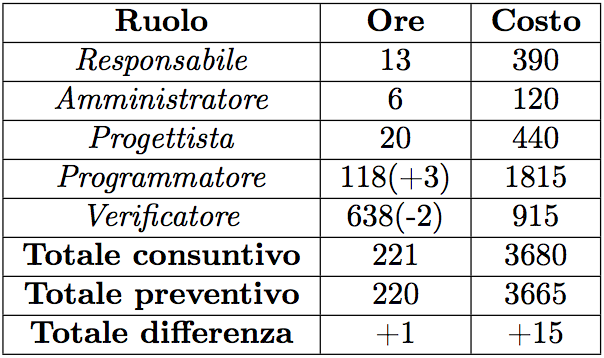
\includegraphics[scale=0.5]{img/prevCD}
  	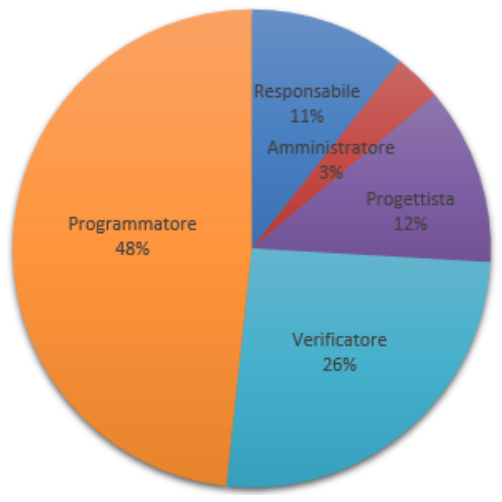
\includegraphics[scale=0.4]{img/cakeCD}
  \end{center}
%Rispetto al preventivo, sono emerse differenze con una diminuzione di 2 ore per il ruolo di Verificatore ed una maggiorazione di 3 ore per quello del Programmatore.
\end{frame}

\begin{frame}
	\frametitle{Preventivo a finire}
	
	\begin{center}
		\centering
		\begin{tabular}{|c|c|}
			\hline
			\textbf{Periodo} & \textbf{Diff} \\
			\hline
			\emph{Analisi dei requisiti}  & 0 \\
			\hline  \emph{Analisi in Dettaglio}  & -15 \\
			\hline  \emph{Progettazione Architetturale}  & +31 \\
			\hline  \emph{Progettazione in Dettaglio}  & +58 \\
			\hline  \emph{Codifica}  & +15 \\
			\hline  \emph{\textbf{Totale}}  & +89 \\
			\hline
		\end{tabular}
	\end{center}
	
Tenendo conto del risultato dei consuntivi nei periodi precedenti, il bilancio totale risulta negativo per 89 \euro.\\

\end{frame}

